\section{V14}
\subsection{Spezielle Eigenschaften des NVIC}\label{NVIC}
\begin{minipage}{9cm}
	Alle Cortex-M Prozessoren enthalten einen \textit{Nested Vectored Interrupt Controller (NVIC)} f"ur das Interrupt-Handling. Neben den klassischen HW-initiierten Interrupts (IRQ) gibt es eine ganze Anzahl von Exceptions, die vom NVIC ebenfalls gehandhabt werden. Dazu geh"oren z.B. Fault Exceptions, NMI Software-Interrupts (SVC), SysTick Timer, usw.
\end{minipage}
%
\begin{minipage}{0.5cm}
	\-\
\end{minipage}
%
\begin{minipage}{9cm}
	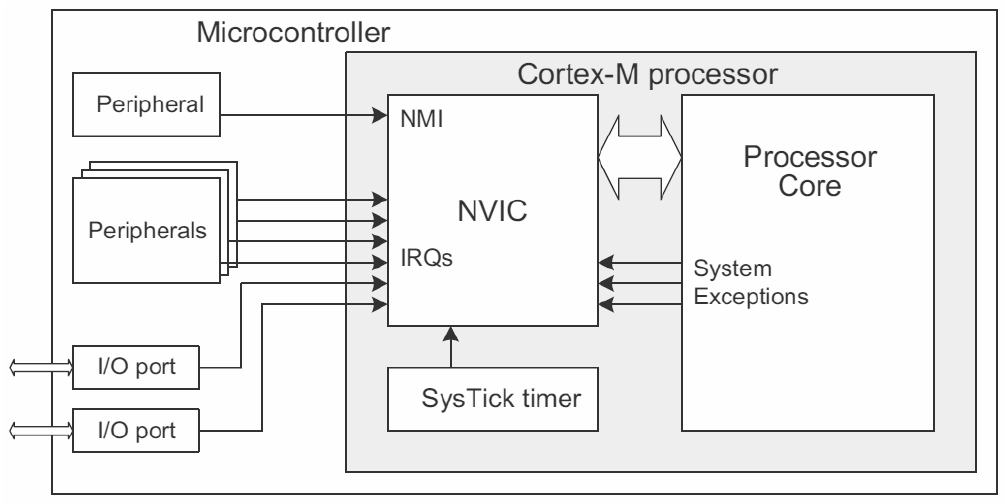
\includegraphics[width=9cm]{images/nvic-cortex-m3} 
\end{minipage}

\subsection{Cortex-M3 Exceptions und Priority-Levels}
\begin{minipage}{9cm}
	Der erste Eintrag in der Vektor-Tabelle (Address-Offset: 0x00) enth"alt immer den Initialwert f"ur den Main Stack Pointer (MSP). Darauf folgt die Einsprung-Adresse f"ur den Reset-Handler. Durchl"auft der Cortex-M seine Reset-Sequenz, so werden diese beiden Eintr"age in den MSP bzw. in den PC geladen. Die n"achsten Eintr"age in der Vektor-Tabelle sind f"ur den Nonmaskable Interrupt (NMI), sowie vier verschiedene Faults reserviert. Weiter oben in der Vektor-Tabelle folgen die
		Adresseintr"age f"ur die weiteren System Exception-Handler.
\end{minipage}
%
\begin{minipage}{0.5cm}
	\-\
\end{minipage}
%
\begin{minipage}{9cm}
	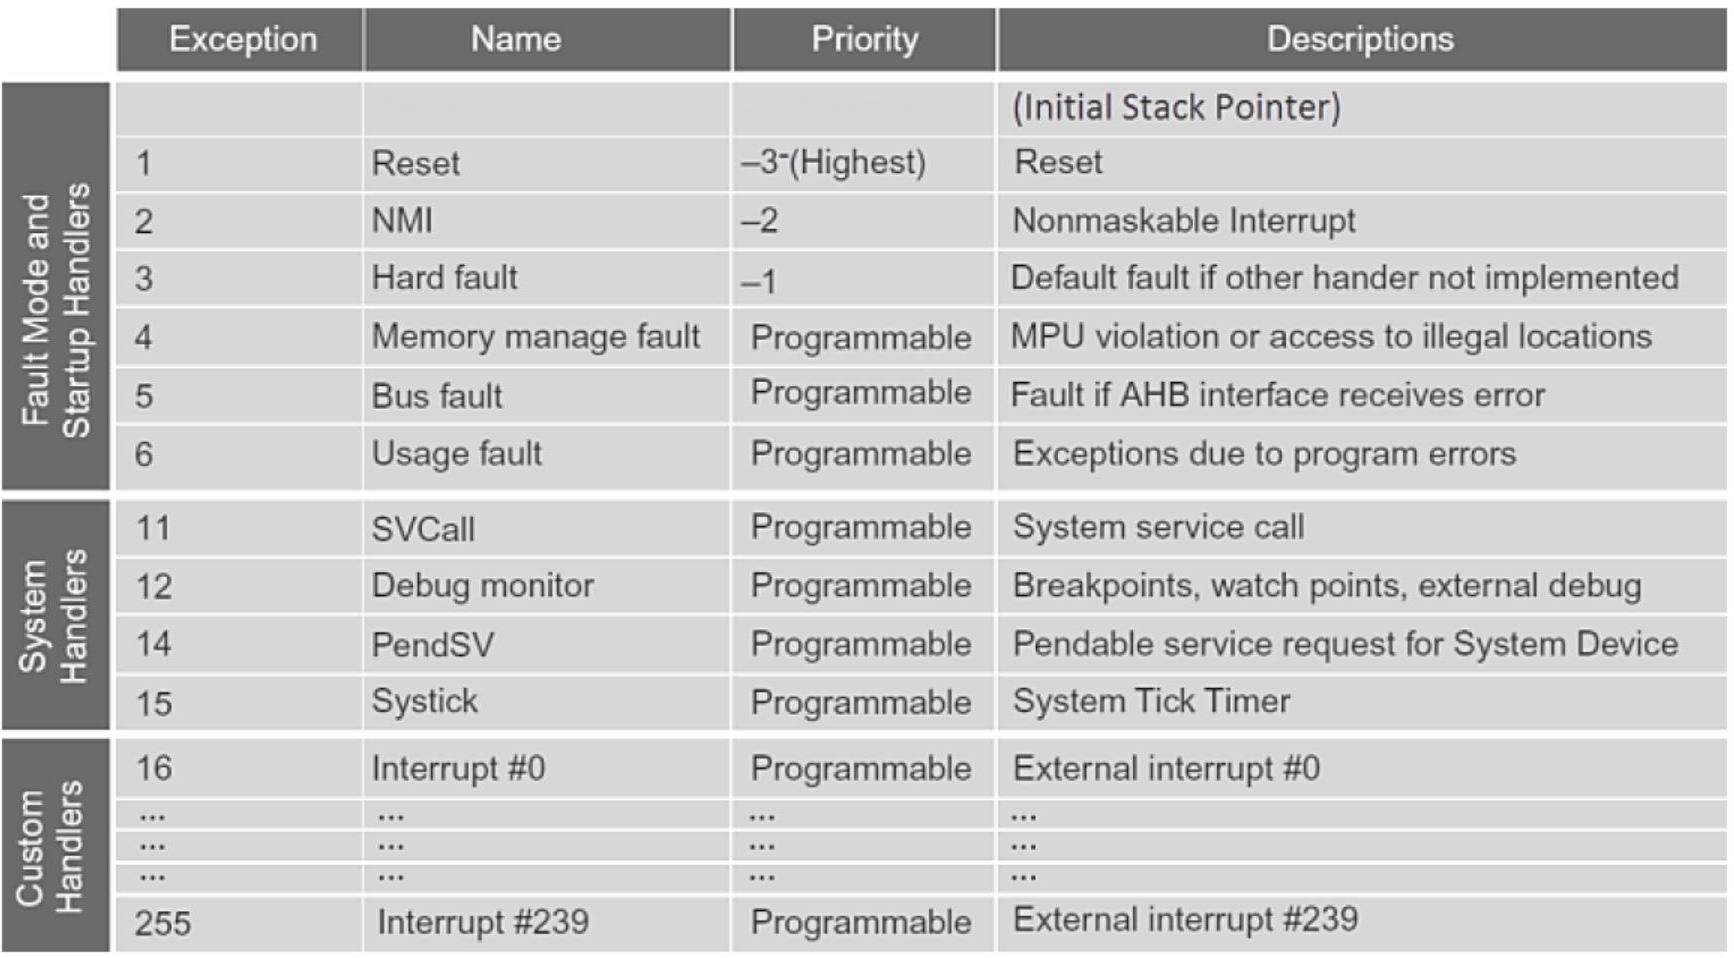
\includegraphics[width=9cm]{images/NVICExcp1} 
\end{minipage}

\vspace{10pt}
\begin{minipage}[t]{9cm}
	\textbf{Usage Fault}\\
	Ein Usage Fault tritt auf, wenn der auszuf"uhrende Application-Code im Cortex-M3 zu einem un"uberwindbaren Fehler f"uhrt. Eine typische Ursache ist beispielsweise, wenn der Prozessor einen ung"ultigen OpCode auszuf"uhren versucht. Weitere Ursachen f"ur einen Usage Fault k"onnte eine Division durch Null sein.\\
	
	\textbf{Bus Fault}\\
	Ein Bus Fault wird ausgel"ost, wenn ein Fehler in der AHB-Bus Matrix erkannt wird. M"ogliche Gr"unde f"ur einen Bus Fault k"onnte eine falscher Memory-Bereich oder eine falsche Gr"osse f"ur einen Datentransfer sein.
\end{minipage}
%
\begin{minipage}[t]{0.5cm}
	\-\
\end{minipage}
%
\begin{minipage}[t]{9cm}
	\textbf{Memory Manager Fault}\\
	Die Memory Protection Unit (MPU) kann in den folgenden F"allen einen Memory
	Manager Fault ausl"osen:\\
	- Accessing an MPU region with the wrong privilege level\\
	- Writing to a read-only region\\
	
	\textbf{Hard Fault}\\
	Ein Hard Fault kann auf zwei Arten auftreten: (1) Wenn ein Bus Fault tritt auf, w"ahrend dem die Vektor-Tabelle gelesen wird. (2) Der Hard Fault wird durch die Eskalationen eines anderen, nicht behandelten Faults aktiviert.
\end{minipage}

\newpage
\subsubsection{Exception-Priority}
\begin{minipage}{9cm}
	Bei den Cortex-M Prozessoren kann individuell festgelegt werden, ob eine Exception zugelassen oder nicht zugelassen werden soll. Dazu wird der aktuelle Priority Level mit der konfigurierten Priority der Exception gegeneinander verglichen. Eine h"oher priorisierte Exception (kleinerer Priority Level) kann eine Exception mit tieferer Priorit"at (gr"osserer Priority Level) unterbrechen. Dieses \textit{preemptive} Verhalten
	wird allgemein als \textbf{Nested Exception/Interrupt Szenario} bezeichnet.\\

Das Priority-Level kann abh"angig vom Modell bis zu 8 Bit gross sein, und kann mit der \textit{Group-Priority} in die \textit{Preempt-Priority} und die \textit{Sub-Priority} aufgeteilt werden. $\Rightarrow$ Festlegung der Anzahl Priority-Level pro Gruppe
\end{minipage}
%
\begin{minipage}{0.5cm}
	\-\
\end{minipage}
%
\begin{minipage}{9cm}
	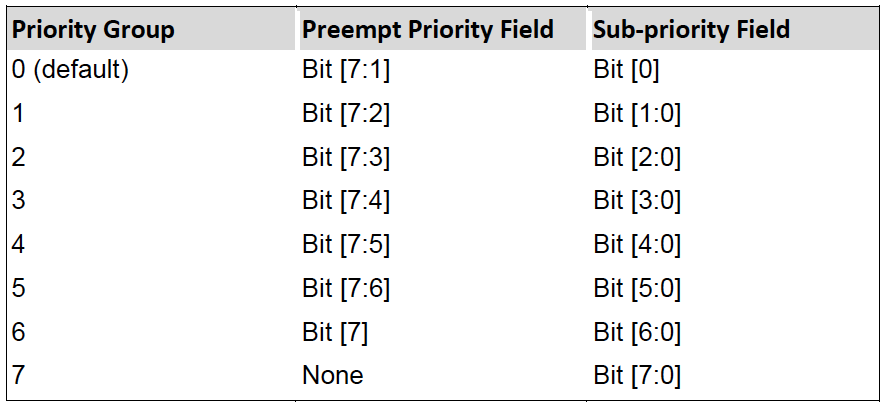
\includegraphics[width=9cm]{images/group-priority}
\end{minipage}


\vspace{10pt}
\begin{minipage}[t]{9cm}
	\textbf{Preempt-Priority}\\
	Legt fest ob ein Interrupt erfolgen kann, wenn bereits ein anderer Interrupt-Handler am laufen ist.
\end{minipage}
%
\begin{minipage}[t]{0.5cm}
	\-\
\end{minipage}
%
\begin{minipage}[t]{9cm}
	\textbf{Sub-Priority}\\
	Wird verwendet, wenn zwei Exceptions der selben Preempt Priority gleichzeitig auftreten. In solchen F"allen wird zuerst die Exception mit der h"oheren Sub-Priority (tieferer numerischer Wert) bearbeitet.
\end{minipage}

\subsubsection{Interrupt-Pending and Activation}
\begin{center}
	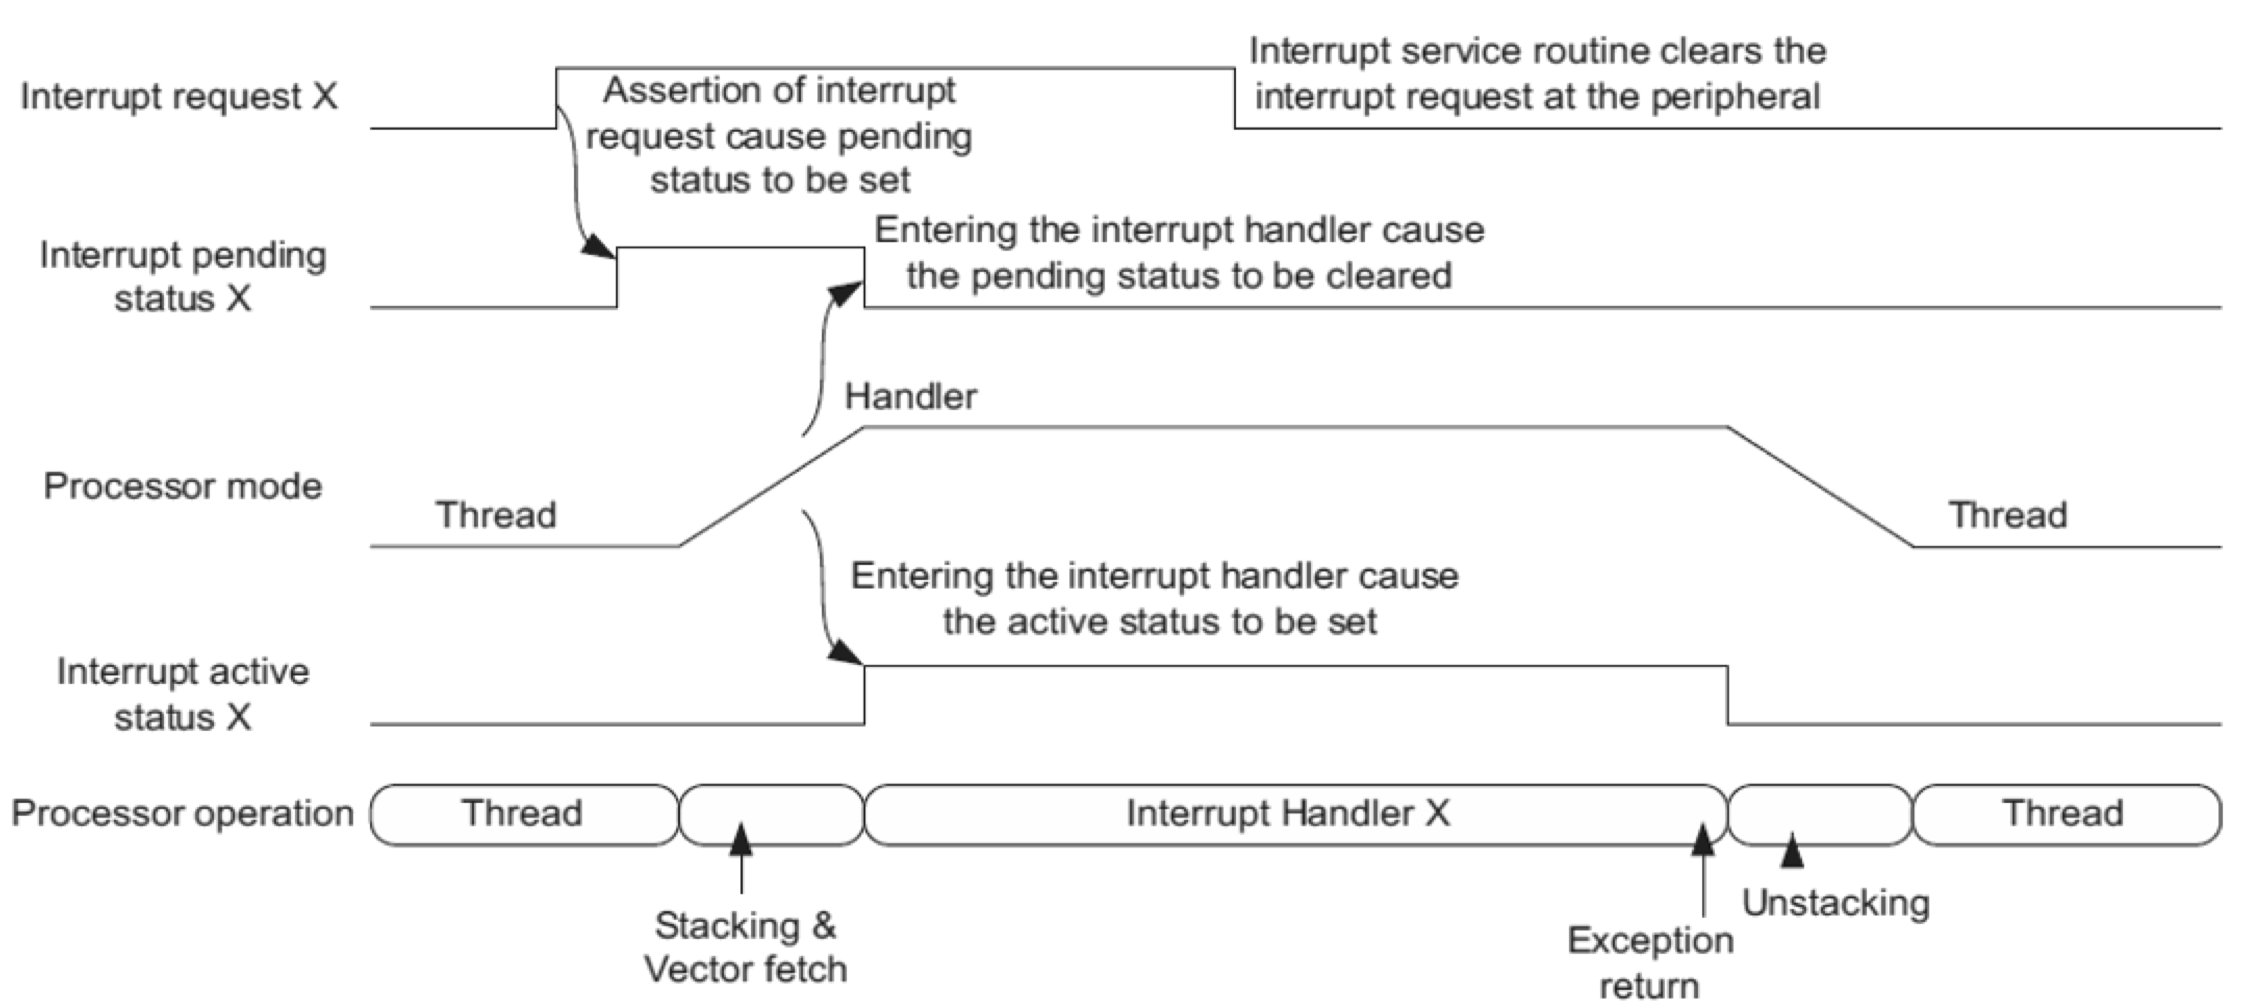
\includegraphics[width=15cm]{images/interrupt-pending}
\end{center}

\subsubsection{Tail Chaining}
Wenn eine Exception auftritt während bereits eine anderen Exception-Behandlung mit gleicher oder höherer Priorität läuft, so wird die neue Exception hinten angestellt. Nach Abschluss des laufenden Exception Handlers, kann die CPU sofort den neuen Exception Request behandeln

\subsubsection{Late arrival}
Wenn der Prozessor einen auftretenden Exceptionrequest akzeptiert, dann startet er die Stacking-Sequenz. Kommt während dem Stacking eine weitere Exception mit höherer Priorität hinzu, so kann diese Late-Arrival-Exception noch bevorzugt behandelt werden.

\subsubsection{POP Preemption} 
Diese Funktion stellt gewissermassen eine Umkehrung des Late-Arrivals dar. Wenn eine Exception Request während dem Unstacking auftritt, so wird das Unstacking abgebrochen, und sofort VectorFetch und Instruction Fetch für den neuen Request durchgeführt. $\rightarrow$ Geschwindigkeitsoptimierung\\

